% DO NOT MODIFY THIS SECTION unless you know what you're doing!z
\documentclass[letterpaper,12pt]{article}

\usepackage{tabularx} % extra features for tabular environment
\usepackage{amsmath}  % improve math presentation
\usepackage{amssymb}
\usepackage{multirow}
\usepackage{xcolor}
\usepackage{gensymb}
\usepackage{appendix}
\usepackage{gensymb}
\usepackage{float}
\usepackage{listings}
\usepackage[export]{adjustbox}
\usepackage{graphicx} % takes care of graphic including machinery
\usepackage[margin=1in,letterpaper]{geometry} % decreases margins
\usepackage{cite} % takes care of citations
\usepackage[final]{hyperref} % adds hyper links inside the generated pdf file
\hypersetup{
    colorlinks=false,       % false: boxed links; true: colored links
    linkcolor=blue,        % color of internal links
    citecolor=blue,        % color of links to bibliography
    filecolor=magenta,     % color of file links
    urlcolor=blue         
}
%++++++++++++++++++++++++++++++++++++++++++++++++++++++++++++++++++++++++++++++++



%++++++++++++++++++++++++++++++++++++++++++++++++++++++++++++++++++++++++++++++++
% Start modifying the labwork number, your team number and the name and METU id
% of your group members.
\newcommand{\reporttitle}{Problem Set 1}
\newcommand{\reportauthor}{ Volkan Aydıngül (Id: 0075359 )\\
                            }
                            % If any teammate does not help to write this report,
                            % you may not write his/her name here.
%++++++++++++++++++++++++++++++++++++++++++++++++++++++++++++++++++++++++++++++++



%++++++++++++++++++++++++++++++++++++++++++++++++++++++++++++++++++++++++++++++++
% DO NOT MODIFY THIS SECTION
\begin{document}
\begin{titlepage}
\newcommand{\HRule}{\rule{\linewidth}{0.5mm}}
\begin{center} % Center remainder of the page
%	LOGO SECTION

\includegraphics[width = 8cm]{figures/koc_logo.png}

%	HEADING SECTIONS
\textsc{\Large PHYS 514 - Computational Physics}\\[1.5cm] 
%	TITLE SECTION
\HRule \\[0.6cm]
{ \huge \bfseries \reporttitle}\\ % Title of your document
\HRule \\[1.5cm]
\end{center}
\vspace{2cm}
%	AUTHOR SECTION
\begin{flushleft} \large
\textit{Author:}\\
\reportauthor% Your name
\end{flushleft}
\vspace{2cm}
\makeatletter
Date: \@date 
\vfill % Fill the rest of the page with whitespace
\makeatother
\end{titlepage}
%++++++++++++++++++++++++++++++++++++++++++++++++++++++++++++++++++++++++++++++++




\tableofcontents
\newpage





%\begin{figure}[H] 
%   \centering \includegraphics[width=\columnwidth]{figures/figure.png}           
%                \caption{Caption}                
%                   \label{fig:label}
%   \end{figure}

\section{Problem I}
\subsection{Calculation of $1 - \frac{\sqrt{1+x^2}}{1+\frac{1}{2}x^2}$}
\paragraph{}In this problem, we are asked to calcute following function:
\begin{equation*}
  f(x) =  1 - \frac{\sqrt{1+x^2}}{1+\frac{1}{2}x^2}
\end{equation*}
\paragraph{} In addition to the calculation, also the minimum precision level of $10^{-8}$ is required. Since we are working on $64 \; bit$ machines, we have always absolute error of $10^{-16}$. First, we need to find the $x$ value which corresponds to border of precision, namely $10^{-8}$. To do that, one can conduct following relation:
\begin{equation*}
   Relative \; Error = \frac{Absolute \; Error}{f(x)}
\end{equation*}

\begin{equation*}
   10^{-8}  = \frac{10^{-16}}{f(x)}
\end{equation*}

Above equation can be solved by \textit{Wolfram Mathematica}, and approximate solution can be found as:
\begin{equation*}
   x \approx 10^{-2}
\end{equation*}

\paragraph{} Now, we know that if the $x$ value drops below $10^{-2}$, we start to lose precision that we wanted. The basic idea behind this situation is the fact that when $x$ is very low, quatioent part starts to approximate $1$ and there happens a loss of signifance due to the $(1-1)$. To deal with this situation, we can expand power series. With help of \textit{Wolfram Mathematica}, one can obtain following power series for $f(x)$.
\begin{equation*}
   f(x) = 0.125x^4 - 0.125x^6 + 0.101563x^8-0.078125 x^{10} + O(x^{12})
\end{equation*}

When we input of $x$ around order of magnitude of $10^{-2}$, we obtain approximately following values:
\begin{equation*}
   f(x) \approxeq 10^{-8} + 10^{-12} + 10^{-16} + 10^{-20} + \dots 
\end{equation*}
We know that criteria to truncate the series for a given precision is:
\begin{equation*}
   \left\lvert \frac{a_{k+1}x_{k+1}}{a_1x_1} \right\rvert < Precision
\end{equation*}
Satisfying above inequality, we deduce that the first three term is sufficient to obtain precision of $10^{-8}$, when the $x$ is lower than $10^{-2}$. Finally, we can write our function in a piece-wise manner as following:

\[ f(x) = 
\begin{cases}
   1 - \frac{\sqrt{1+x^2}}{1+\frac{1}{2}x^2} & x\geq 10^{-2} \\
   0.125x^4 - 0.125x^6 + 0.101563x^8 &  x < 10^{-2} \\
      
\end{cases} 
 \]

 The \textit{loglog} plot that represents the $f(x)$ can be seen in Figure \ref{fig:loglogb}.

 \begin{figure}[H] 
   \centering 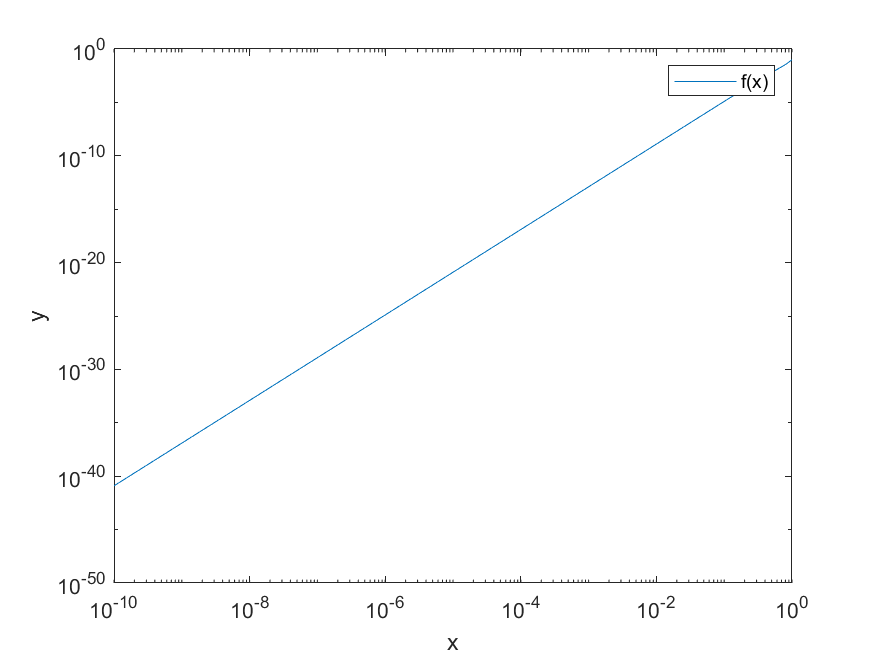
\includegraphics[width=\columnwidth]{figures/loglogb.png}           
   \caption{Loglog plot of $f(x)$}                
   \label{fig:loglogb}
   \end{figure}



 \subsection{Calculation of $\cot x^2 - \frac{1}{x^2}$}
 \paragraph{}Again, in this problem, we will exactly apply above procedure. In this case, our function is:
 \begin{equation*}
   f(x) =  \cot x^2 - \frac{1}{x^2}
 \end{equation*}
 \paragraph{} First, we need to find the $x$ that corresponds to loss of precision of $10^{-8}$. Again, by using \textit{Wolfram Mathematica}, we find that:
 \begin{equation*}
    Relative \; Error = \frac{Absolute \; Error}{f(x)}
 \end{equation*}
 
 \begin{equation*}
    10^{-8}  = \frac{10^{-16}}{f(x)}
 \end{equation*}
 
 \begin{equation*}
    x \approx 10^{-4}
 \end{equation*}
 
 \paragraph{} Let's expand power series with help of \textit{Wolfram Mathematica}:
 \begin{equation*}
    f(x) =-\frac{x^2}{3}-\frac{x^6}{45}-\frac{2 x^{10}}{945}-\frac{x^{14}}{4725}-\frac{2 x^{18}}{93555}+O\left(x^{21}\right)
 \end{equation*}
 
 When we input of $x$ around order of magnitude of $10^{-4}$, we obtain approximately following values:
 \begin{equation*}
    f(x) \approxeq 10^{-8} + 10^{-24} + 10^{-40} + 10^{-56} + 10^{-80} + \dots 
 \end{equation*}
 We know that criteria to truncate the series for a given precision is:
 \begin{equation*}
    \left\lvert \frac{a_{k+1}x_{k+1}}{a_1x_1} \right\rvert < Precision
 \end{equation*}
 Satisfying above inequality, we deduce that the first term is sufficient to obtain precision of $10^{-8}$, when the $x$ is lower than $10^{-4}$. Finally, we can write our function in a piece-wise manner as following:
 
 \[ f(x) = 
 \begin{cases}
   \cot x^2 - \frac{1}{x^2} & x\geq 10^{-4} \\
   -\frac{x^2}{3} &  x < 10^{-4} \\
       
 \end{cases} 
  \]
 
  The \textit{loglog} plot that represents the $f(x)$ can be seen in Figure \ref{fig:loglogc}.

  \begin{figure}[H] 
    \centering 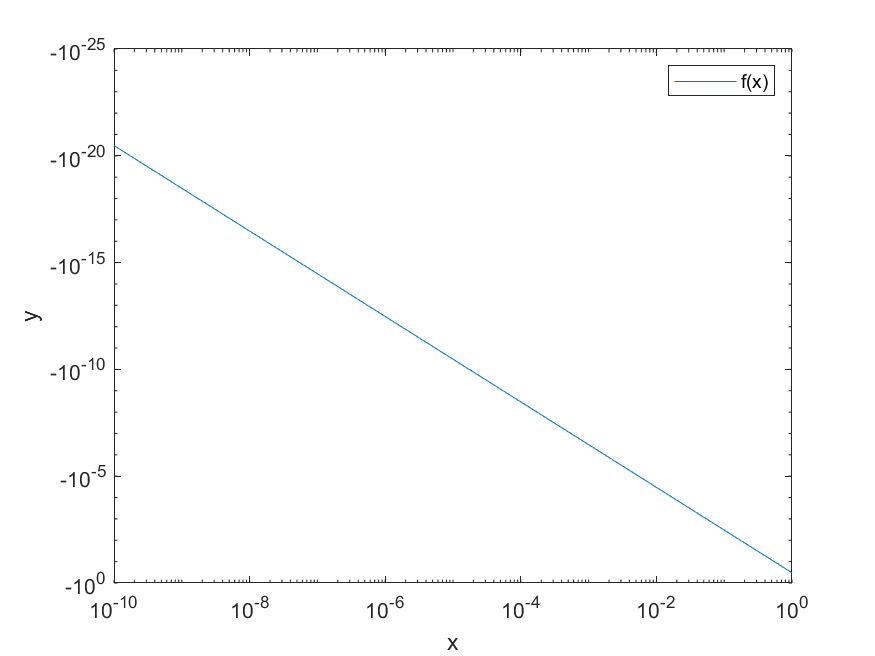
\includegraphics[width=\columnwidth]{figures/loglogc.png}           
       \caption{Loglog plot of $f(x)$}                
                    \label{fig:loglogc}
    \end{figure}




\section{Problem II - Roots of Quadratic Equation}
\paragraph{}Let's illustrate the quadratic equation, 
\begin{equation*}
   ax^2 + bx + c = 0
\end{equation*}
In this case, the roots of the above equation can be defined as follows:
\begin{equation*}
   x_{1,2} = \frac{-b \pm \sqrt{b^2 - 4ac}}{2a}
\end{equation*}
\paragraph{}However, when we use above form for root finding, some problems may occur. One of these problems is that when the difference between the terms $b^2$ and $4ac$ is very large, the loss of significance may take place. For example, when $c$ is very small, depending on the sign of the $b$, the aforamentioned loss of significance can reduce the accuracy dramatically. In essence, the more stable algorithm which eliminates the usage of substraction is needed.
\subsection{Alternative Form for Root Finding}
\paragraph{}In alternative method, the purpose is to eliminate the need for substraction, which is the main source of the loss of significance. When $a$ or $c$ is very small compared to the $b^2$, the square term is very likely to result in very close value to $b$. In this case, ultimately, we need to process following calculation:
\begin{equation*}
   -b + b^*
\end{equation*}
where $b^*$ stands for \textit{very close number to $b$}. To get rid of the catastrophic cancellation that may occur due to the above calculation, we can use below formula to calculate the one of the roots.

\begin{equation*}
   x_{1} = \frac{-b - sgn(b)\sqrt{b^2 - 4ac}}{2a}
\end{equation*}

By doing that, we can only encounter with either summation of two positive numbers or summation of two negative numbers. Finally, the second root can be calculated as follows:
\begin{equation*}
   x_{2} = \frac{c}{a x_1}
\end{equation*}

The formula to find second root is simply derived from the \textit{multiplication of the roots} relation:
\begin{equation*}
   x_1x_{2} = \frac{c}{a}
\end{equation*}

\pagebreak
\section{Problem III and IV}
When we apply the asked procedure the estimate the average round-off error of summing the all elements in an array of $n$ elements, we obtain the following Figure \ref{fig:normalloglogsum}:

\begin{figure}[H]
   \centering
   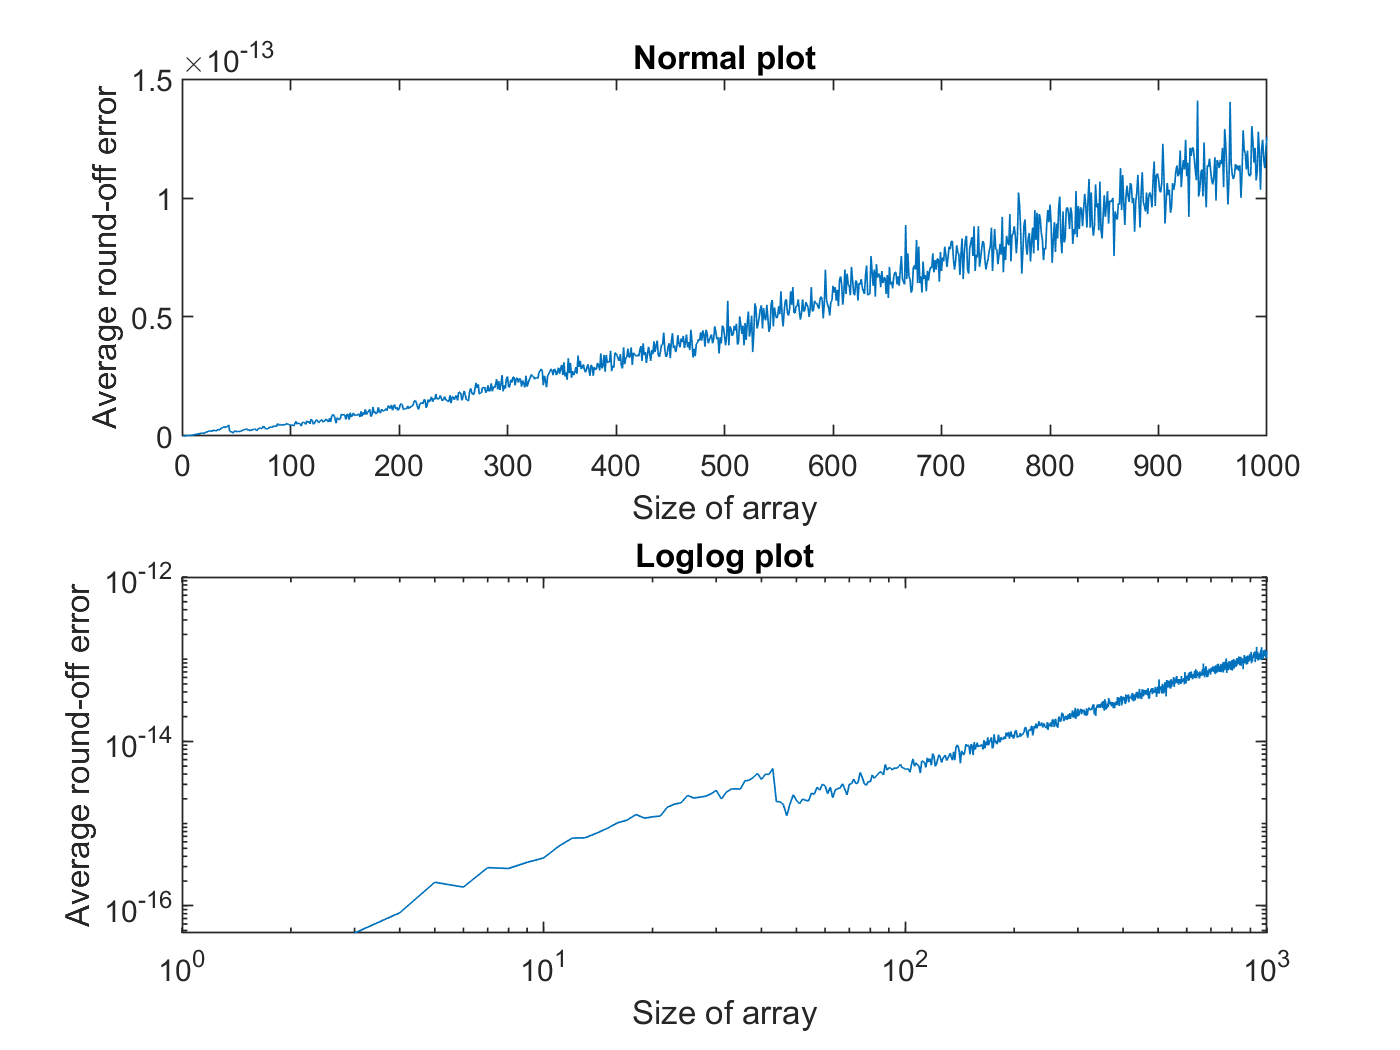
\includegraphics[width=\linewidth]{figures/normalloglogsum.png}
   \caption{Normal and Loglog plot for MATLAB $sum$ function}
   \label{fig:normalloglogsum}  
   \end{figure}

   \paragraph{}Observing the figures, from the $loglog$ plot, we can clearly see that there is a exponential trend in the growth of error. However, due to the easily observed noise in the Figure \ref{fig:normalloglogsum}, it can be deduced that estimate of the average round of error displays a random walk with respect to size of array. Ultimately, we can conclude that even though the error is small, it can accumulate and grow exponentially with the size of array.

   \paragraph{}To overcome this loss of accuracy, we can employ \textit{Kahan summation}, which is used to minimize the loss of significance. It achieves that by storing a seperate variable which holds the cumulative error.
   \pagebreak
   \paragraph{}In this way, the round-off error can reduce significantly, which can be seen from Figure \ref{fig:normalsumKahan}.


\begin{figure}[H] 
   \centering 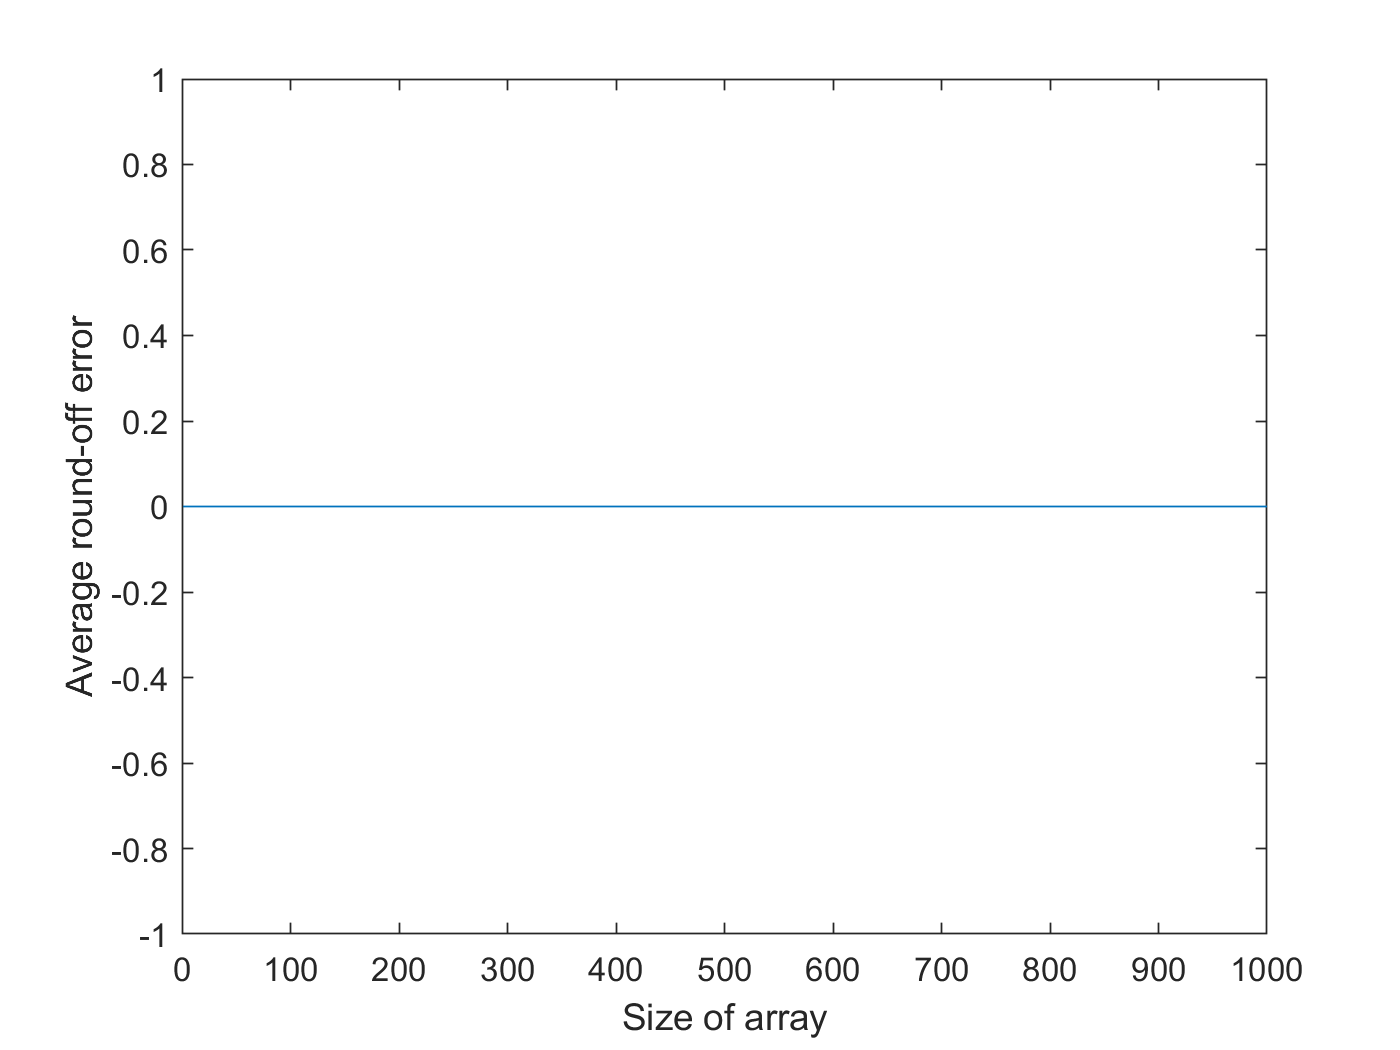
\includegraphics[width=0.5\columnwidth]{figures/sumKahan.png}           
                \caption{Normal plot for custıom $sumKahan$ function}                
                   \label{fig:normalsumKahan}
   \end{figure}

   \paragraph{} However, even this algorithm can fail in certain ill-conditioned situations. For example, this algorithm is tend to lose its capability to have very small round-off error when the inputted array does not consists of numbers having mean of zero. In below Figure \ref{fig:kahanill}, we can observe that error is not stable around $0$, when the input array consists of number having mean of $3$ (normal distribution).
\begin{figure}[H] 
   \centering 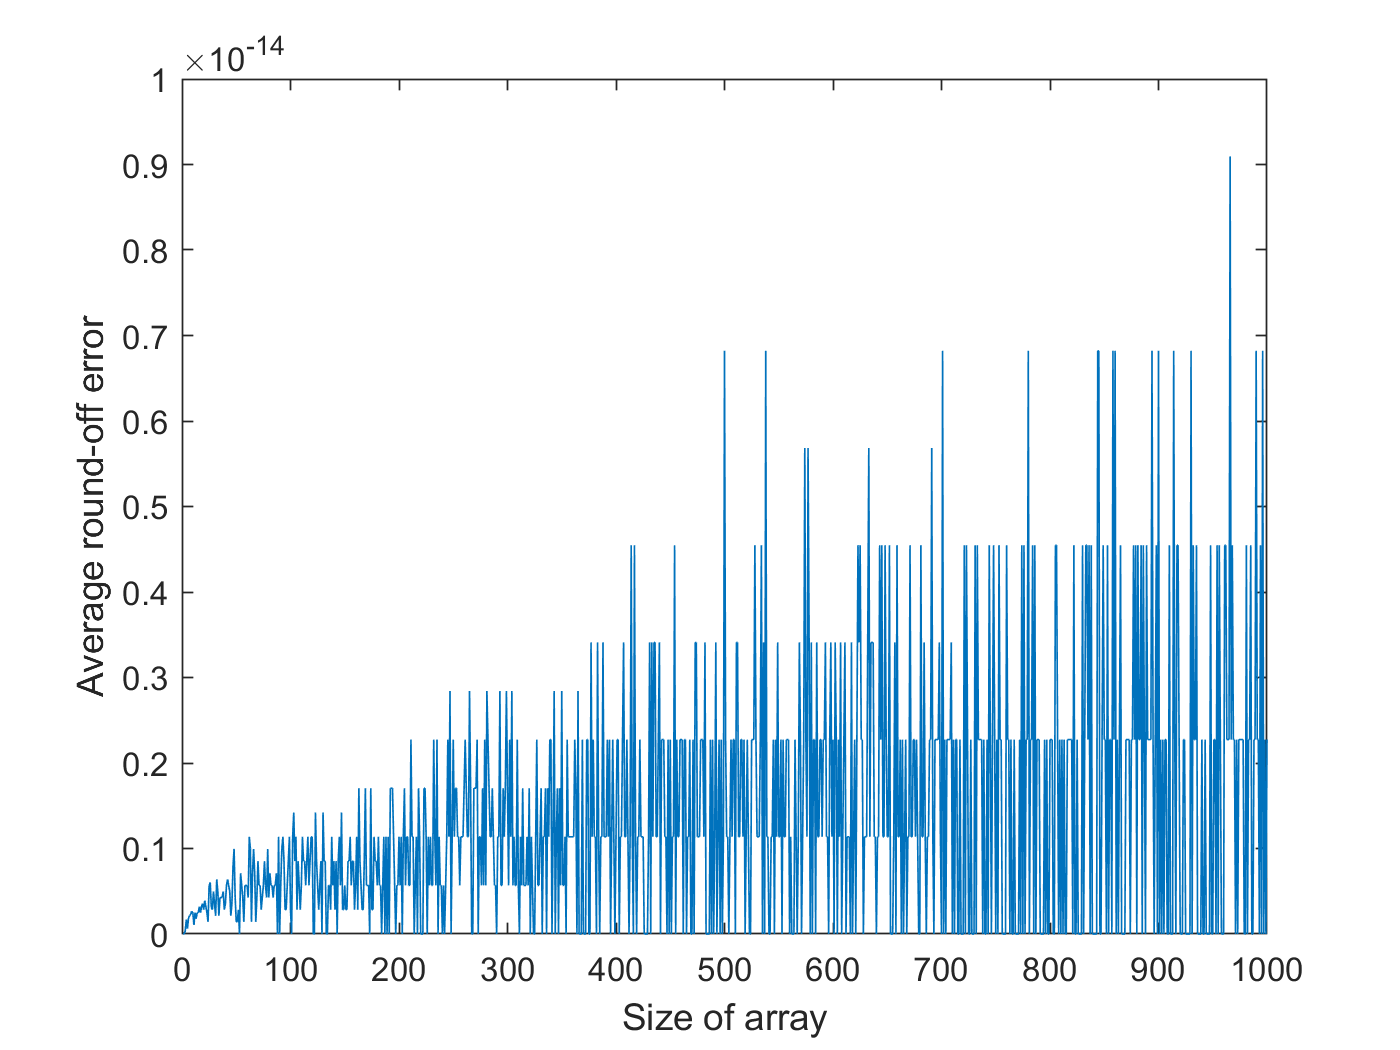
\includegraphics[width=0.7\columnwidth]{figures/kahanill.png}           
                \caption{Ill-condition case for Kahan Summation}                
                   \label{fig:kahanill}
   \end{figure}
\end{document}

              


